% Configurações gerais
    \documentclass[twoside, 12pt, english,italian,latin,greek,french,spanish,brazil]{book}
        \usepackage{Arvo}
        \usepackage[T1]{fontenc}
        \usepackage{enumitem}
        
    % Language setting
    % Replace `english' with e.g. `spanish' to change the document language
    \usepackage[portuguese]{babel}
    \renewcommand{\thesection}{\arabic{Seção}}
    \renewcommand{\thechapter}{\arabic{Capítulo}}
    \addto\captionsbrazil{\renewcommand{\sectionname}{Parte}}

    % Set page size and margins
    % Replace `letterpaper' with `a4paper' for UK/EU standard size
    \usepackage[a4paper,top=3cm,bottom=2.5cm,left=3cm,right=3cm,marginparwidth=1.75cm,portrait]{geometry}

    % Useful packages
    \usepackage{amsmath}
    \usepackage{graphicx}
    \usepackage{caption}
    \usepackage[colorlinks=true, allcolors=blue]{hyperref}

    % Beggining 


    \title{MORPHOADEQUABILITAS: \\ \small{O Projeto de Traçados Urbanos sob Nova Perspectiva}}

% Título anterior: {A PROJETAÇÃO DE TRAÇADOS URBANOS EM NOVA PERSPECTIVA: \\ \small{O Conceito de Rendimento Urbano desenvolvido como Método de Projeto para (Novas) Áreas Urbanas morfologicamente adequadas ao Sítio}}

\author{Higor Ribeiro da Costa}

        \usepackage{setspace}
    
\begin{document}
    \maketitle
    \setstretch{1.15}
    \setcounter{secnumdepth}{1}

\begin{abstract}
        \textbf{Abstract} \\
Como projetar novas áreas urbanas morfologicamente adequadas ao sítio? Que é possível traçá-las, é fato: é possível observar isso seja nas cidades espontâneas como em algumas cidades pré-concebidas. Porém, em suas expansões, muitas dessas cidades apresentam novas áreas urbanas com características dessemelhantes e qualidade inferior ao traçado original. E o que se observa é que não há um caminho pelo qual se orientar no sentido de desenvolver novos traçados urbanos morfologicamente ade-quados ao sítio e congruentes em sua lógica interna. Logo, a questão não é saber ‘se é’ possível, mas ‘como’ desenvolvê-los.  Para responder a essa questão, na presente tese desenvolve-se um método de projeto baseado no conceito de ‘rendimento urbano’ – oriundo do desenvolvimento e adaptação de conceitos da escola italiana de morfologia urbana, e definido como a coerência intrínseca entre o traçado da forma urbana e o contexto natural, aferível por parâmetros como coerência, organicidade, hierarquização, limitação e continuidade de percursos. Essa pesquisa é desenvolvida por meio de \textit{Evidence Based Design}. E, para isso, traçados urbanos são projetados com base nos parâmetros do rendimento e nas características morfológicas de sítios escolhidos co-mo amostras, sendo comparados com traçados urbanos existentes e não-adaptados ao sítio em termos das qualidades advogadas aos traçados morfologicamente adequados. Disso, são deduzidos passos projetuais a serem seguidos metodicamente. E tais passos, dispostos à guisa de método, são validados por grupos focais de pesquisadores, estudantes e profissionais que seguem tais passos de modo a de verificar se tal método é aplicável nos diferentes contextos da realidade. Diante disso, tal tese é estruturada em quatro capítulos: a revisão do estado da arte acerca do tema principal e daquilo a ele correlacionado; a projetação, comparação e análise dos traçados; a proposta e os resultados dos grupos focais; e, por fim, o resultado esperado, colocado como quarto capítulo, é um manual com diretrizes e diagramas para a projetação de novas áreas urbanas. (312 palavras). \\
\textbf{Keywords:}
\textit{Urban Morphology; Urban Design; Urban Growth; New Urban Areas; Urban Sustainability.} 
\end{abstract}

\newpage

\section{Introdução}
    \maketitle

    %% Comentários Instrumentalização da Tese 2023-03-24:
        % Prof.ª Gislaine:
            % Problemática: levantar variáveis como 'sustentabilidade', etc. (que mencionei na apresentação e que possivelmente vão fazer parte do desenvolvimento do método). Logo, é necessário CONTEXTUALIZAR melhor a problemática.
            % Método ≠ Manual
            % Foco: [Se for] método, ele é:
                % Descritivo?
                % [É] Um programa de computador?
            % Você fala muito em 'topografia' e 'manual', mas isso está superado 'a meu ver'. 
            % [Logo,] O que de inédito tem na sua tese?
        % Prof. Sidnei: 
            % Topografia
            % Sistematização
            % É possível que já exista um estado da arte que abranja isso que você quer tratar
            % Menção a design guides ingleses – o prof. Renato deve conhecer melhor que eu, mas é muito útil você fazer menção a isso no seu projeto [/introdução].
    
    %% Comentários Pós-aula Instrumentalização da Tese 2023-03-29 (Gislaine Beloto):
        % "Faça como o Vitor [Oliveira]: crie uma teoria e vá ser famoso." — "Não se preocupe tanto com o método; isso virá em breve, na própria disciplina".
        % "\textit{DSR} virou método da moda – essa era a crítica de um artigo que [eu, G.B.] li".
        % Minha tese, "justamente, pode ser a questão do conceito 'morfoadequado' [sic]" — "se eu coloco [o termo morfoadequabilidade ou morfoadequado] no 'problema', eu não tenho mais tese [,eu não tenho mais do que falar]."
        % "[Pior que seu trabalho dá para uma teoria, mas não vou falar assim para não te dar bola]

    \subsection{Apresentação do tema}	

    Há muito que me pergunto o porquê de nossas cidades serem tão feias. 'Se temos tanta tecnologia hoje, porque construímos casas, prédios, bairros e cidades assim?' Tenho passado anos com essa dúvida perseguindo meu pensamento e, em parte, é por essa razão que escrevo a presente tese. Posso afirmar com Philippe Daverio que as nossas cidades, sobretudo nossas novas áreas urbanas, são feias.\footnote[1]{Daverio (2022, \textit{s.p.}) fala das periferias da cidades italianas, utilizando-as, eu diria, como um estudo de caso. No fim, ele fala das áreas de expansão urbana, o que, em nosso caso, corresponde a áreas com novos loteamentos, sejam eles contínuos ou contíguos à mancha urbana existente, ou mesmo a novos loteamentos inseridos em vazios urbanos, como glebas remanescentes de um processo de especulação, o que não configura, necessariamente uma periferia. Ademais, o termo 'periferia' costuma evocar a ideia de periferia social, o que, no caso de um traçado urbano, poderia ser materializado por uma favela. Porém, tanto eu quanto Philippe Daverio %(VÍDEO DO DAVERIO FALANDO SOBRE MATERIA, SOBRE O BELLO IN CITTÀ, FALANDO DELE NO RIO E FALANDO QUE AS FAVELAS SÃO LINDAS COMO PRES~EPIOR  COMO PRES~EPIOS NAPOLITANOS E QUE NEAS SÓ NÃO HÁ A CATEDRAL E O CASTELO DO NOBRE)
     estamos de acordo que as favelas são 'bonitas', e isso precisamente por seu aspecto morfológico.} Elas suscitam um juízo estético transversal quase que unânime. Talvez 'feiúra' não seja o que melhor define nossas cidades, muito embora \textit{“mentre sul bello si fatica a trovare un parametro congiunto, sul brutto sembra essere meno problematico trovare un terreno comune.”} (DAVERIO, 2022, \textit{s.p.}).\footnote[2]{'Enquanto tem-se dificuldade para encontrar um parâmetro conjunto para [o termo] 'belo', em relação [ao termo] 'feio' parece ser menos problemático encontrar um terreno comum' (tradução nossa).} Desse modo, ao invés de falar em 'feiúra' ou 'beleza', falarei simplesmente de 'harmonia' – falarei disso no momento oportuno.
     
     Voltemos à retórica pergunta inicial. Penso que, em relação às edificações em geral, temos uma explicação na obra de Gianfranco Caniggia e Gian Luigi Maffei (2008 [1979], pp. 50-57) com dois conceitos fundamentais: \textit{'tipo'} e \textit{'rendimento'}. Basta, por ora, dizer que o \textit{rendimento} é, no caso das edificações, a medida da coerência entre o \textit{tipo} de uma edificação individual e o \textit{tipo} presente nas construções ao seu redor; e que o \textit{tipo} é 'o produto da consciência espontânea radicada no imaginário coletivo, formado pelo universo de elementos físicos ao nosso redor' (COSTA, 2020, p. 43), \textit{i.e.}, o conjunto de características que está presente em cada edificação, ainda que essas edificações não sejam idênticas. Desse modo, quanto mais cada nova edificação '‘se render’ ao \textit{tipo} do ambiente, [assumindo] as características comuns do contexto onde é colocada' (COSTA, 2020, p. 44), maior o seu \textit{rendimento} – e, portanto, maior a harmonia do conjunto. Se isso não resolve a situação em relação às edificações, ao menos a atenua, na medida em que confere maior coesão, e, portanto, harmonia ao conjunto.

     Porém, se temos uma solução em relação às edificações – quero dizer, temos ao menos um vislumbre do que fazer –, o mesmo não se dá em relação ao traçado urbano. E aqui faz-se necessário elucidar a diferença entre duas dimensões a que devemos atentar ao analisar essa as cidades. A primeira é a sua '\textit{forma},' aquilo que podemos enxergar diretamente com os olhos e apalpar com mais facilidade na cidade – isto porque a \textit{forma} urbana (\textit{the urban form}) é, por definição, tridimensional, eu diria até 'mais material'. A segunda dimensão é o 'traçado urbano' (\textit{the urban shape}), o 'formato' da \textit{forma,} o contorno que a delineia, o que, por definição, é bidimensional, e, por isso mesmo, 'menos material', ou seja, perceptível pelos sentidos apenas de maneira latente e apenas observável por meio de um processo de abstração que envolve a apreensão da \textit{forma} e sua posterior representação. Representação essa mais esquemática e abstrata do que o seria uma representação direta da \textit{forma} – basta pensar na diferença entre uma pintura (como as de Caspar van Wittel) 
     \ref{fig:exemplo}
      e um mapa (como o de Giambattista Nolli). %QUAL A DIFERENÇA ENTRE TRAÇADO E FORMA, DE VERDADE? ISSO SÃO AUTORES OU VEM DA ETIMOLOGIA, SÃO CONCEITOS QUE PEGO DE ALGUÉM, OU EU QUE ESTOU CRIANDO A DISTINÇÃO?

    \begin{figure}[h]
        \centering
        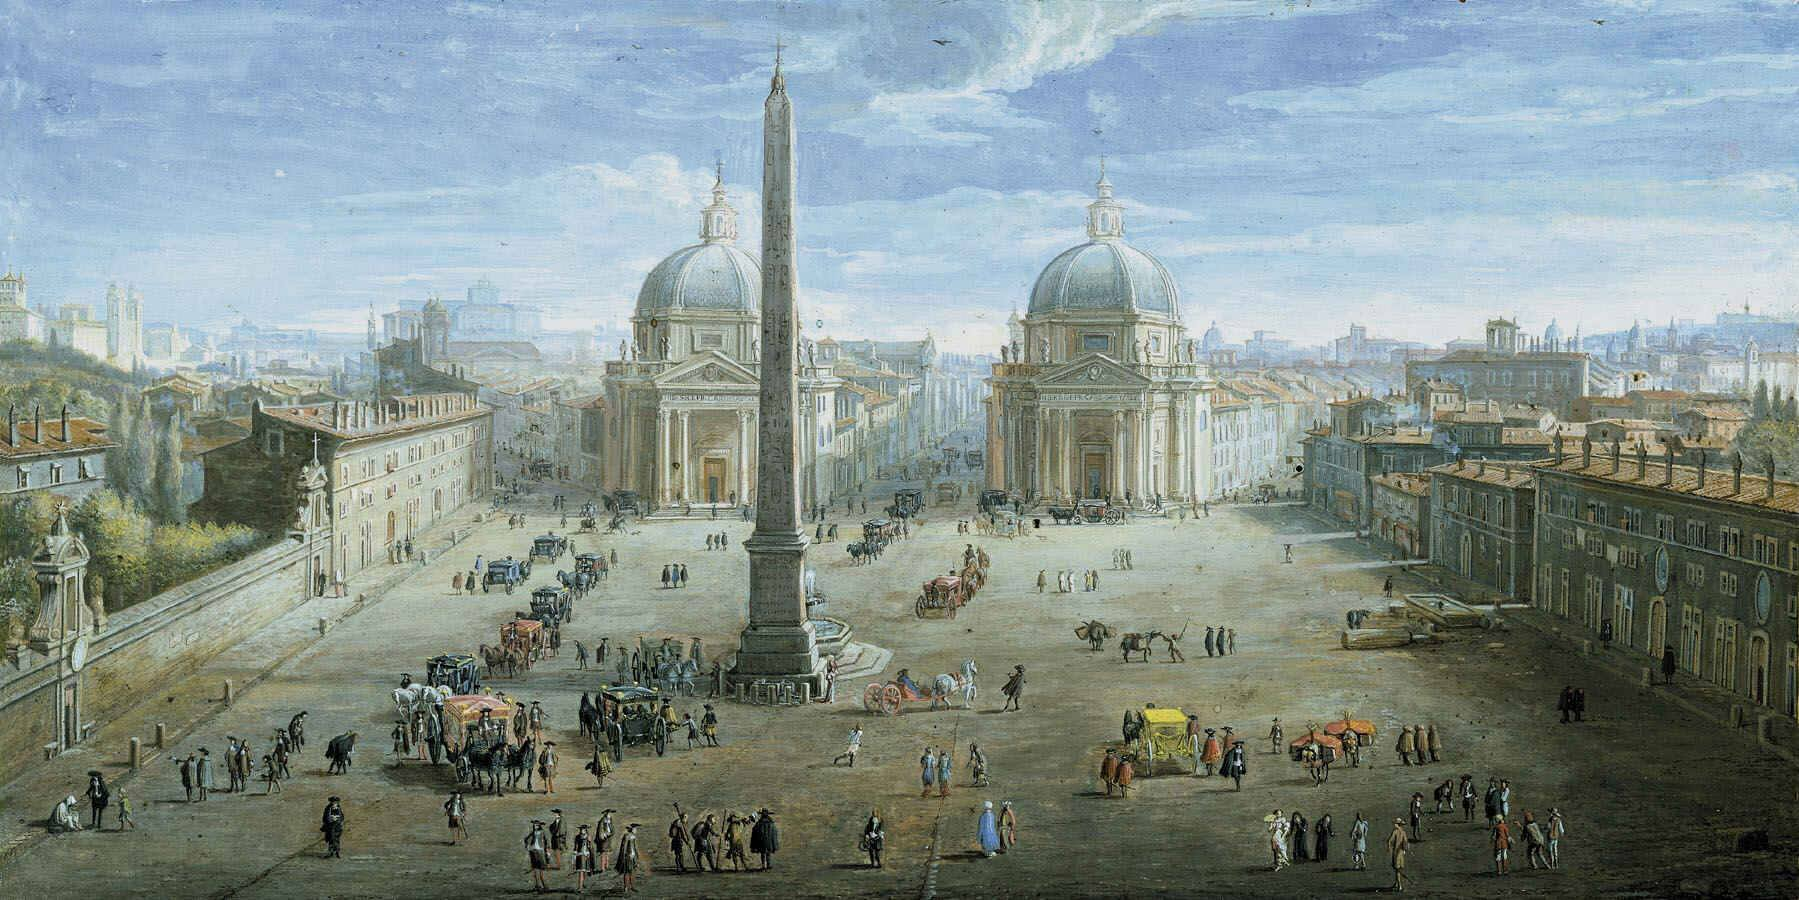
\includegraphics[width=1\textwidth]{Pictures/popolo.jpeg}
        \label{fig:exemplo}
        \captionsetup{labelfont=bf}
        \caption{Vista da \textit{Piazza del Popolo}, em Roma, por Caspar Van Wittel (1652–1736). \textbf{Fonte:} Wikimedia Commons / Sotherby's (coleção privada).}
    \end{figure} 

    Discorramos rapidamente sobre a ideia de \textit{forma} e traçado. Traçado é o particípio do verbo traçar, \textit{i.e.,} desenhar traços, riscar, sendo o ato ou efeito desse mesmo verbo, resultando, portando, em um 'conjunto de traços', ou, no nosso caso, no 'desenho que representa uma estrutura arquitetônica ou urbanística', o que é equivalente a dizer 'planta', 'projeto', ou, para usar um termo mais antigo, 'traça' (PRIBERAM, TRAÇADO, 2023). Na língua rústica do latim, 'tracto' que dizer 'traçar sulcos', e 'tractus' é a 'delimitação por meio de traços; região, lugar, quarteirão' (FARIA, 1962, p. 1010). Penso que não haja melhor definição que essa: 'delimitação por meio de traços' – que corrobora com a ideia de trajetória de estrada ou linha férrea (PRIBERAM, TRAÇADO, 2023). \textit{Forma,} porém, é um termo mais complexo.
    
    \textit{Forma} é a 'configuração das coisas na parte exterior', o que é equivalente a 'feitio' e 'formato' (PRIMERAM, FORMA, 2023). No latim, a coisa complica um pouco, com \textit{'forma'} querendo dizer 'fôrma' (que em português é um 'molde sobre o qual ou dentro do qual se coloca alguma substância fluida, que toma o feitio desse molde'), ou 'todo objeto feito na fôrma'; pode, de fato, ser entendida como 'desenho, modelo, planta', mas também pode ser entendida como 'tipo ideal', ou ainda como 'conformação, configuração, constituição' (FARIA, 1962, p. 407). E, se formos para o campo da filosofia, aí é que a confusão aumenta, pois temos um 'sentido filosófico e particularmente metafísico', um 'sentido lógico', outro 'epistemológico', um metodológico', e, por fim, ainda um 'sentido estético' (MORA, 2001b, p. 1126) – e, portanto, a ideia de \textit{'forma'} escapa-nos neste momento.
    %Ao tratar do termo "morfoadequado", deve-se mencionar que, em estética 'o termo 'forma' também é utilizado na estética para designar a ordem na qual estão dispostos os elementos em um conjunto (por exemplo, para falar de simetria). [E] Nesse caso a forma não se contrapõe ao conteúdo' (MORA, 2001b, p. 1130).
    %'Classicamente se considerou que uma obra de arte deveria ter uma 'boa forma'; a isso se chamou \textit{formosus}­, do que deriva 'formoso'. O que \textit{formosus} ou bem proporcionado opõe-se ao disforme, freqüentemente identificado ao que é feio.' (MORA, 2001b, p. 1130). Juntando isso ao que fala Daverio sobre o conceito grego de que algo é belo quando tem uma utilidade faz-nos (faz-me) pensar que um traçado urbano – hoje – só é belo, formoso, harmônico, quando cumpre sua função, ou melhor, o programa programático de funções a que deve cumprir [e] em coerência com a topografia [e demais estruturas naturais e antrópicas que dela derivam].
        %Agora... Qual é esse programa de funções que um traçado urbano deve cumprir? É ser a base dos lotes? É ser o conjunto de vias que possibilita o tráfego de pessoas, veículos, etc., de modo a criar a economia da cidade (ALAIN BERTAUD) e sua lógica social (BILL HILLIER) enquanto, ao mesmo tempo, mantém QUALIDADES relativas ao imaginário coletivo (CARVALHO), à Thigmotaxis (SUSSMAN) (mantendo o senso de orientação na cidade, seja ela em relação aos percursos a que seguir, seja em sentido mais profundo, de oikophilia, no qual eu me identifico com o lugar, sabendo 'de onde vim e para onde vou' na existência e no tempo (PETERSON)? Seria esse o complexo programa de um traçado urbano? Seria mais simples? Ou seria mais complexos e com outros desdobramentos, como conduzir (ou ser reflexo) de políticas de preservação e recuperação do meio ambiente (seja daquele existente em escala regional – como fundos de vale e cunhas verdes – como daqueles destinados ao lazer dos cidadãos – como parques, praças, chegando aos canteiros), e tudo isso sem esquecer do aspecto de minimização dos impactos relacionados ao assoreamento dos rios e expansão urbana sobre área rural (AUTORES?), bem como do aspecto social de garantir acesso aos centros à força de trabalho (BERTAUD) de maneira equânime (HARVEY?). Tudo isso é um grande escopo a ser estudado.
        %% TUDO ISSO CONSTITUI A 'PARS PRIMA' DO TRABALHO, PRECEDENDO AO MÉTODO (PRÁTICO) DE PROJETO DE NOVOS TRAÇADOS URBANOS ENQUANTO PERFAZ O CONCEITO DE 'MORFOADEQUABILIDADE' DE UM TRAÇADO URBANO (TEORIA): OU SEJA, O QUE UM TRAÇADO URBANO DEVE SER E COMO EU O PROJETO.

    Desse modo, na presente pesquisa, utilizo o termo 'traçado urbano' para me referir sobremaneira ao desenho das vias (\textit{open spaces}),\footnote[3]{\textit{'The public spaces system of a city includes (...) the open spaces for movement, which we designate, in a simplified way, as streets, (...) [and] also the open spaces for permanence, which we designate as squares and gardens.'} (OLIVEIRA, 2016, p. 17).} ainda que o termo 'traçado urbano' também faça referência aos lotes, quarteirões e contornos edificados (que, não raro, definem o próprio desenho das vias, por meio da conjunção de fachadas).\footnote[4]{Note-se que, diferente do que atualmente é lugar comum, o que definia o que era ou não a rua, seu limite, seu contorno, seu espaço, era precisamente a fachada da edificação, que imprime essa linha ao mesmo tempo imaginária e real no solo, diferente do que ocorre hoje. Hoje, o lugar comum é aquele de que o que define a via é o meio-fio. E isso é fruto da desvinculação entre edificação e lote, entre os limites da edificação e os limites do lote. Mas, se olharmos para nosso passado urbano, veremos algo bem diferente. Basta olharmos uma pintura de Caspar Van Wittel da \textit{Piazza Navona} em Roma e veremos como a praça já era muitíssimo bem definida (pelas edificações), mesmo sem qualquer indício de calçamento, e muito menos de meio-fio.} Outrossim, quando penso em 'vias', compreendo sua relação com 'nós' urbanos abertos, como praças, e nós urbanos 'cobertos' ou 'fechados', como equipamentos com acesso franqueado ao público, como igrejas, \textit{shoppings} e galerias – desde que com características morfológicas análogas às 'vias' e 'nós' urbanos abertos, o que será elucidado apropriadamente mais adiante. % CHECAR STRAPPA (1995) NA QUESTÃO DOS NÓS URBANOS. O QUE É UM NÓ URBANO, COMO ELE SE CONFIGURA COM O NÓ NATURAL, COMO É UM NÓ ARQUITETÔNICO, QUAL O TERMO CORRETO, SE ELE SEMPRE ESTÁ CORRELACIONADO COM UM NÓ NATURAL (cf. CANIGGIA & MAFFEI, 2008), ETC.







    %Olavo de Carvalho
    %Conceito de beleza (citar também 'formosus' (DAVERIO, 2022; MORA, 2001b, p. 1130).
        %De pulchrum et de bonum (Santo Tomás) que traduz 'καλόν τε καί αγαθόν' dos gregos (o belo e o bom) (SEVIER, 2012, p. 17), citado por Daverio: o belo sendo aquilo que agrada aos olhos (sentidos?) e o bom sendo aquilo que se relaciona com algum fim. καλοκαγαθία 
            %ST I.5.4 ad 1. Ad primum ergo dicendum quod pulchrum et bonum in subiecto quidem sunt idem, quia super eandem rem fundantur, scilicet super formam, et propter hoc, bonum laudatur ut pulchrum. Sed ratione differunt. Nam bonum proprie respicit appetitum, est enim bonum quod omnia appetunt. Et ideo habet rationem finis, nam appetitus est quasi quidam motus ad rem. Pulchrum autem respicit vim cognoscitivam, pulchra enim dicuntur quae visa placent.
    %Conceito de harmonia (Checar Suma Teológica)
    %Tipo
    %Rendimento

    %% O projeto de um traçado urbano é análogo ao que, em música, chamamos de 'variações sobre um tema'. Estas nada mais são que (...). Dito isso, tomemos como exemplo as 'Seis Variações em Ré Maior, Op. 76,' de Beethoven – recomendo a performance no piano de Cédric Tiberghien. Nela, temos sete partes: o tema principal e as seis variações. 
    %Primeiro, o tema principal. Segundo, uma variação refinada, delicada, que preenche o esqueleto do tema principal. Terceiro, uma mescla do tema principal, mais grossolano e do segundo. Quarto, um tema delicado, assim como o segundo, com pinceladas suaves sobre o tema inicial, à semelhança do que faz a segunda variação. Quinto, uma brincadeira criativa com as variações precedentes, mostrando os contornos dos músculos assentados sobre os ossos do tema inicial. Na sexta, a pele, a última cobertura delicada a se aplicar ao corpo de variações. E, por fim, na sétima peça, a sexta, última, e mais longa variação, uma complexa construção resultante de todas as variacoes, do esqueleto do tema à pele suave do corpo, assim como o traçado com suas edificações harmoniosamente assentadas sobre o sítio. Assim deve ser o projeto de um traçado urbano. Um vai e volta que sempre observa o tema principal dominante – o relevo, a topografia, as estruturas naturais do sítio – ao mesmo tempo em que agrega a ele elementos antrópicos: percursos, ruas, quadras, edificações, musculatura ao esqueleto, gerando um conjunto coeso que, no fim, ainda revela a estrutura inicial, assim como um corpo humano deixa entrever sua estrutura óssea por meio do seu formato.

        %\textit{{'$\mu$}{$o}{$\rho\phi$}{$ή}'} (morfé) e {$\textit{adaequabilitas}}, forma e adequabilidade.
        \textit{Morfé} e \textit{adaequabilitas}, forma e adequabilidade.
        Adequabilidade da forma (da forma do traçado do traçado às formas do substrato), ou adequabilidade à forma (adequação da forma do traçado, ou do traçado, à forma do substrato).

        Como projetar novos traçados urbanos morfologicamente adequados ao sítio de maneira metódica? Em minha dissertação (COSTA, 2020), pude verificar que é possível projetar novos traçados urbanos adequados às características orográficas de um sítio, gerando, outrossim, parâmetros para a avaliação desses traçados. Porém, uma coisa sou eu projetar um traçado urbano dentro de um contexto acadêmico. Outra coisa são outros estudantes a efetuar a mesma tarefa sem o mesmo cabedal. Mais ainda, uma coisa é o \textit{Quartiere Quinto} em Gênova, de Gianfranco Caniggia (Figura 1); e outra coisa são os loteamentos que surgem à medida que nossas cidades se expandem atualmente. São duas \textit{formae mentis} distintas, dois modos de projetar diversos, dois \textit{modi faciendi} completamente diferentes. De uma parte, aqueles que partem da apreensão da realidade material antes do projeto;  de outra aqueles que têm uma concepção apriorística do que realizar, e que só fazem pequenos ajustes no esquema mental ao confrontá-lo com a realidade. Em ambas as situações, porém, e principalmente na primeira, a \textit{forma mentis} é fruto de um saber construído de maneira complexa, quase que por tradição – ainda que aprendida na universidade – e pouco dela se tem sistematizado como método, e menos ainda de maneira automatizada. %ESCREVER QUE 'MODUS FACIENDI' É ANÁLOGO A 'FORMA MENTIS', I. E., UMA ESTRUTURA MENTAL. 

         É verdade que na obra de Gianfranco Caniggia e Gian Luigi Maffei (2008) temos o \textit{vade mecum} da escola italiana de tipo-morfologia, no qual estão descritos conceitos e métodos de leitura de edificações, tecidos e organismos urbanos e territórios, afinal o nome da obra é \textit{“Lettura dell’edilizia di base”}. No entanto, projetar um traçado urbano ex novo requer olhar para essa obra pelo avesso, e, com base em tudo o que nela se pode aprender, projetar um novo traçado urbano – e só isso já ultrapassaria uma tese. O que se pretende aqui é algo mais modesto: desenvolver um método de projeto de traçados urbanos morfologicamente adequados ao sítio. A ideia é fornecer à comunidade acadêmica e profissional – envolvendo pesquisadores, professores, alunos, além de arquitetos, engenheiros, agrimensores e outros técnicos do setor público e privado – um manual de projeto de traçados urbanos. E, com isso, almeja-se ainda colaborar com o debate acerca da morfologia urbana – que passa transversalmente da arquite-tura ao planejamento territorial, passando pelo urbanismo e pela geografia, e desde condomínios fechados até favelas –, gerando uma alternativa ao \textit{modus faciendi} atual e franqueando o acesso ao arcabouço teórico-metodológico da escola italiana de tipo-morfologia.

        A presente tese, portanto, nada mais é que a continuação da pesquisa iniciada no mestrado.  Na dissertação, desenvolvi o conceito de “rendimento urbano” (COSTA, 2020; COSTA E REGO, 2019), desdobramento do conceito de \textit{“rendimento”} da escola italiana de morfologia urbana,   adaptando-o para a escala da cidade a partir de sua aplicação na escala edilícia (CANIGGIA E MAFFEI, 2008, pp. 52-53) e do território (CARLOTTI, 1995, pp. 17-19). De maneira geral, o \textit{rendimento} é o “grau de coerência com o contexto” (MAFFEI, 2003, p. 82, tradução nossa). Assim, o rendimento edilício é o grau de coerência entre o tipo  de uma edificação e o tipo das edificações já existentes no conjunto no qual ela é inserida (CANIGGIA E MAFFEI, 2008, p. 52; CATALDI, 2003, p. 31). Enquanto isso, o rendimento territorial é a disposição de um território para a utilização do homem,  em atividades como deslocamento, habitação, produção agrícola e produção urbana – sendo medida pela geomorfologia e pela localização geográfica de uma determinada área  (CARLOTTI, 1995). 

        Adaptado para a escala da cidade, o rendimento urbano foi definido como a “coerência intrínseca entre o traçado da forma urbana e o contexto natural” (COSTA, 2020, p. 47). Essa noção indica que o traçado urbano deve ser consoante ao sítio, particularmente à sua topografia, e que isso deve se dar de tal maneira que esse traçado seja hierarquizado e unitário, com elementos e arranjos interdependentes. E, desenvolvida essa noção, cinco parâmetros foram desenvolvidos para avaliar traçados urbanos. São eles a “coerência”, a “organicidade”, a “hierarquização”, a “limitação” e a “continuidade de percursos” (COSTA, 2020, p. 83). Verificou-se ainda que tais parâmetros ser-vem não apenas à avaliação do rendimento de um traçado urbano, senão que serviam ainda à projetação de novas áreas urbanas, servindo como balizadores de projeto. 

        A partir disso, desenhei um traçado urbano sobre uma porção já ocupada de Maringá – a Zona 20 –, de modo a verificar se um traçado urbano baseado no rendimento era viável – a ao menos em teoria (Figura 2). E isso em termos de desenho, de cumprimento da normativa de áreas mínimas, do fornecimento e distribuição de espaços e equipamentos públicos e de viabilidade econômica, com uma quantidade razoável de lotes vendáveis – o que se mostrou possível. Fiz a comparação entre o traçado desenhado e aquele existente na área e cheguei à conclusão de que um traçado urbano baseado no rendimento é superior aos traçados atuais, feitos com \textit{offsets} dos limites dos lotes rurais nos quais os loteamentos são inseridos, ao mesmo tempo que são viáveis. Mas tudo isso ‘em teoria’, haja visto que esse traçado foi projetado sobre uma grande área que funcionou como uma folha em branco – semelhante ao que ocorreu com o plano original de Maringá, projetado por Jorge de Macedo Vieira. No entanto, o resultado poderia ser diferente se o parcelamento rural, segmentado como era, tives-se sido levado em conta sem esse \textit{land readjustment} virtual que a pesquisa anteriormente permitiu.
 
        \caption{Figura 2: Relação de percentuais legais entre o traçado existente e o traçado projetado. Fonte: COSTA, 2020, p. 111.}

    \subsection{Problemática}

        De fato, novos traçados urbanos podem ser desenvolvidos coerentes com o relevo, com elementos organicamente interdependentes, hierarquizados, delimitados e mais ou menos pervasivos, a depender de seu papel e importância no conjunto. Eu mesmo testei isso face a um traçado já consolidado. Todavia, algumas lacunas relacionadas ao rendimento urbano ainda precisam ser exploradas. O processo de formação de conjuntos edificados, cidades e territórios foi devidamente descrito e pormenorizado por Gianfranco Caniggia e Gian Luigi Maffei (2008 [1979]); e, a partir de seus estudos, chega a ser possível propor novas edificações, bairros ou mais. E tudo isso com critérios científicos – incorporados à arte do projetar, como ficou provado no \textit{Quartiere Quinto}, em Gênova (Figura 1). Porém, há coisas que permanecem sem solução.

        A primeira é que, se os lotes, quarteirões e bairros podem seguir uma lógica de crescimento orgânico (CANIGGIA E MAFFEI, 2008), existe algo ainda mais ‘primitivo’, a saber, “não existe assentamento sem um percurso [pré-existente]” (CANIGGIA, 1976, p. 69, tradução nossa). Hoje, projeta-se a quadra para depois se pensar no lote e na rua (isso não é um processo necessariamente diacrônico, mas é a \textit{forma mentis} mais em voga). Ao contrário do que se vê em nota mais espontâneas, em que o percurso prece-de a conformação dos organismos urbanos – da edificação à metrópole (Figura 3)–,   hoje o que se percebe é que o percurso é deixado em segundo plano.

        Com efeito, um conjunto edificado possui, em seu processo de formação, condicionamentos às suas formas, como as irregularidades do relevo. É sobre esse relevo que se assentam os percursos nos quais se apoiam parcelamentos e edificações por meio dos quais se organizam cidades e territórios (CANIGGIA, 1976, p. 69-72; CANIGGIA E MAF-FEI, 2008, pp. 209-212). Já vimos que é possível projetar traçados de acordo com o sítio. Porém, e em segundo lugar, a lógica de identificação de onde um percurso deve ou não passar ainda está ‘no olho’ do projetista – e pode acabar não seguindo uma lógica orgânica, consoante ao relevo. Não mais vivemos na época em que, para abrir um caminho, bastava soltar um jumento para que ele, buscando os pontos mais fáceis de atravessar na topografia, indicasse por onde deveria seguir a picada. Não. Vivemos em uma época em que se exige um planejamento que congregue diversos projetos, feitos por profissionais com base em saberes técnicos. Todavia, não há um método ou ferramenta para guiar estudantes e profissionais na tarefa de projetar um traçado urbano (seja um novo traçado ou uma intervenção) tão adequado ao relevo quanto não o fazia um jumento. Não há um passo-a-passo para projetar traçados segundo o arcabouço teórico da escola italiana de tipo-morfologia, particularmente a partir do conceito de rendimento. Sem isso, permanece o \textit{modus faciendi} atual impresso no traçado urbano, que, uma vez consolidado, torna-se praticamente impossível de ser alterado (REIS FILHO, 2000). 

        Por terceiro, mas não menos importante, ao tratar de método de projeto, fala-se necessariamente de processo. Porém, o conceito inicial de rendimento, do qual o rendi-mento urbano não é senão desdobramento – como um membro de um corpo –, só seria aplicável à avaliação de um ‘antes’ e um ‘depois’ (CANIGGIA E MAFFEI, 2008, pp. 51-52), “em função do tempo e das obras necessárias às adaptações do contexto à intervenção”. Dessa maneira, mesmo que o rendimento não impeça de “verificar a qualidade do processo em si” (COSTA, 2020, pp. 45-46), o termo torna-se restritivo no momento em que busco desenvolver um método de projeto – ainda que baseado nesse conceito. E, com isso, faz-se necessário desenvolver um novo termo que conceitue de modo sintético tudo aquilo que busco exprimir com a expressão bilíngue “rendimento urbano”.

    \subsubsection{\textit{Modus faciendi}}

        Um adendo aqui se faz necessário, e é sobre o termo \textit{modus faciendi}, que emprego \textit{ad nauseam} em minha pesquisa. \textit{Modus faciendi} quer dizer basicamente ‘maneira’ ou ‘modo de fazer’ algo. É análogo ao modus operandi. Porém, enquanto a expressão \textit{‘modus operandi’} geralmente trata do comportamento das pessoas, a expressão \textit{‘modus faciendi’} aqui trata da maneira como alguém faz algo: que passos segue, que resultados obtém e quais as características desse resultado. E, em se tratando de morfologia urbana, é possível elencar ao menos três variáveis do \textit{modus faciendi} atual.

        A primeira e mais comum é o traçado baseado em um esquema de ‘grelha’. Vias retas e cruzamentos ortogonais. Nele, o desenho das vias não se adequa ao desenho das curvas de nível, logo, não há vias curvas; no máximo, o que ocorre é um direciona-mento da reta no sentido da declividade e do escoamento da água. O traçado pode ser um \textit{grid} totalmente ortogonal (a 90°), com quadras quadradas ou oblongas; ou pode ser uma ‘árvore’, em que os percursos menores desaguam em um percurso principal do qual derivam, como uma ‘espinha de peixe’, sem formar cruzamentos, mas sim gerando desencontros entre as vias. E seus limites e disposição interna geralmente são dados pela replicação paralela – ou \textit{offset} – da linha que perfaz o limite da gleba rural do loteamento ou de algum percurso precedente, ou mesmo de alguma outra linha de força, que pode ser motivada pelo próprio relevo, ainda que não se adeque a ele em seu formato retilíneo. Essa é a variável que mais se pode verificar nos loteamentos construídos país afora, posto que sua vantagem para um empreendedor individual reside na praticidade de rapidamente projetar o empreendimento e vender os lotes, de modo a viabilizar empreendimentos sucessivos que ele precise custear. A vantagem, porém, termina por aí, pois para o usuário final a questão pode ser um pouco mais complicada, seja a nível intramuros que na escala urbana (de movimentação de terra a dificuldade de implementação de modais de transporte público que atendam a todas as classes sociais).

        A segunda é o traçado de esquema ‘ameboide’, \textit{i. e.}, com vias curvas, mas nem sempre adequadas ao relevo de maneira satisfatória. Esse esquema carece de organicidade, posto que as vias não derivam umas das outras a partir de uma hierarquia coerente com o relevo do sítio. Ao contrário, são apenas curvas ‘soltas’, ‘lúdicas’ – para usar um termo tão caro aos arquitetos da moda –, que servem para tornar o ambiente mais agradável e o tráfego mais tranquilo enquanto a sucessiva promenade de casas desenhadas à moda de programas de televisão fechada se desenrola aos olhos deleitados do observador desprovido de algum senso crítico. Esse esquema, diferente do esquema em ‘grelha’ a \textit{offset}, geralmente não atende a pequenos proprietários de lotes rurais, que precisam fazer um empreendimento apenas após quitar o anterior. Ao contrário, os traçados ameboides, via de regra, são utilizados em grandes empreendimentos, i. e., os ditos ‘condomínios fechados’ com alto valor agregado, geralmente associados a um status social elevado graças à imagem de exclusividade passada pelo marketing do empreendimento. São traçados fechados e não raro com apenas uma única conexão com o restante da cidade, causando uma segregação morfológica severa, ao separar trechos da cidade que poderiam estar conectados, ou ainda, pro-movendo o espraiamento urbano, na medida em que são construídos fora dos limites da cidade. A falsa realidade à parte da verdadeira realidade – pena que se fale tanto do aspecto social sem referência à morfologia desses traçados, posto que a condição sociológica que os gera vai muito além do alcance da arquitetura, embora possa ser mitigado materialmente – morfologicamente – por esta.

        A terceira é o esquema orgânico de rápida expansão desordenada. O melhor exemplo disso são os assentamentos informais, como as favelas. Neles, é possível verificar a estruturação dos percursos edificados – matriz, implantação e coligação – sobre ruas que seguem as formas do relevo do sítio em que se implantam. Porém, como não raro esses traçados ‘surgem’ apenas da necessidade imediata de habitação por parte de populações carentes, que ocupam áreas ociosas no território urbano (como interstícios urbanos, encostas e fundos de vale) próximas de centralidades urbanas,  o que ocorre é a materialização de um traçado urbano orgânico, mas insuficiente. Orgânico no sentido de interdependência e hierarquização dos percursos – sobretudo se os observarmos de maneira ‘abstrata’, partindo apenas dos eixos das vias. E insuficiente porque dada a necessidade premente de habitação em pontos estratégicos atrair um grande fluxo de pessoas (AUTOR???), o que ocorre é a ‘apropriação’ – ou ocupação, assenta-mento –, por exemplo, de áreas cada vez mais íngremes (nas encostas) ou alagáveis (nos fundos de vale), impróprias para a construção pois passíveis de desastres ambientais, sobretudo dada a fragilidade das construções e a impermeabilização do solo nas cidades (também oriunda da falta de entendimento sustentável do traçado urbano, onde se aplica a ideia de rendimento, como tratada na dissertação). Outrossim, por conta dessa mesma motivação e sem alguém que guie esse processo – a figura do ‘príncipe’, como diria Philippe Daverio – os percursos apresentam apenas as dimensões mínimas para a circulação de pessoas, sendo verdadeiros corredores e não ruas. É de notar que isso não põe em demérito o traçado desses assentamentos, mas mostra que é necessário dar um guia e balizamento para seu crescimento, caso ele ocorra, visto seu potencial: primeiro paisagístico, posto que essas comunidades apresentam uma identidade forte graças à presença de um tipo distinguível em suas edificações,  dispostas sobre percurso hierarquizados em coerência com o relevo graças a um fazer espontâneo; segundo por conta da economia das cidades (BERTAUD, 2018), posto que tais comunidades usualmente se colocam onde há proximidade de áreas em que é possível obter emprego a uma distância razoável, diminuindo o tempo – nesse sentido, tais áreas podem receber os benefícios de uma maior integração com o traçado da cidade existente e vice-versa.

        Reservo-me a não comentar os experimentos de regimes totalitários, dentre os quais a capital brasileira representa o maior expoente. Uma vez que há a abolição da cidade, do organismo urbano, do quarteirão e do próprio edifício (graças à ausência de \textit{footprint} gerada pelos pilotis), em vista da dissipação das massas em caso de manifestações frente a um Estado centralizador, não há o que comentar de tais cidades de um ponto de vista morfológico. Mais interessantes são as favelas e bairros crescidos ao redor dessas excrecências urbanas do que o seu ‘traçado’ em si.

    \subsection{Hipóteses e questões}	 

        A partir da dissertação de mestrado desenvolvida anteriormente (COSTA, 2020), podem-se deduzir duas hipóteses, uma subordinada à outra. E cada uma delas traz questões principais e questões derivadas. Essas, por sua vez, dão origem aos objetivos e motivação à escolha do objeto, como se verá mais adiante.

        A primeira hipótese é a de que é possível projetar novos traçados urbanos morfologicamente adequados ao sítio. Corroboram com essa hipótese o próprio \textit{Quartiere Quinto} em Gênova, de Caniggia, já mencionado (CATALDI et al., 2014), o \textit{Piano per le Barene di San Giuliano} em Veneza, de Saverio Muratori (MARETTO, 2013; OLIVEIRA, 2021), o próprio ‘Ante-projeto’ para Maringá, projetado por Jorge de Macedo Vieira – ainda que feito sobre outras bases teóricas (BONFATO, 2008; REGO, 2001, 2009; REGO et al. 2004); e ainda o próprio traçado que desenvolvi durante o mestrado (COSTA, 2020). 

        Partindo dessa primeira hipótese surge a seguinte questão: como projetar novos traçados urbanos morfologicamente adequados ao sítio por meio de um método? E, a partir disso, a seguinte questão derivada: esse método serve – ou deve servir – para todos os contextos (situações reais) ou apenas para algumas situações específicas? Por exemplo: 
        \dots
            \begin{itemize}
                \item Servirá só para casos \textit{ex novo} (como no Plano Vieira e no traçado da dissertação)? 
                \item Servirá para situações com \textit{land readjustment}?
                \item Ou também servirá para situações previamente parceladas?
                    \subitem Com um parcelamento urbano prévio?
	                Com um parcelamento rural prévio?
	                    \subsubitem Segmentado em pequenas propriedades, como as da CTNP?
                        \subsubitem Ou também com outras configurações, com glebas maiores?
            \end{itemize}

        Já a segunda hipótese, subordinada à primeira, é a de que existem traçados urbanos morfologicamente melhores e piores. A questão é: traçados urbanos são melhores ou piores sob quais aspectos? Um traçado em grelha com \textit{offset}, por exemplo, é proveitoso para quem deseja economizar com tempo, recursos humanos e infraestruturas, além de lucrar com maior facilidade; mas não é proveitoso para o usuário final (proprietário) e para a sociedade. O empreendedor economiza ao pagar profissionais sem \textit{savoir-faire} específico durante menos tempo por um projeto simples e comum, feito no quotidiano de um escritório que precisa de muitos desses pequenos projetos para se manter. Além disso, com lotes projetados com formatos estritamente ortogonais, o processo de demarcação é (aparentemente) mais simples, a venda é mais rápida, a contabilização de áreas é mais prática e o registro em cartório é (aparentemente) mais célere. Mas os benefícios param por aqui. Os contras são a ‘mono-tonia’, a dificuldade em evitar declives graças ao desenho forçosamente retilíneo que pouco ou nada se adapta à pendência pluvial, e, como consequência do desenho do traçado, muitas vezes a necessidade de movimentação de terra no sentido de lateral a lateral do lote se faz presente, com ladeiras nas ruas que tornam difícil o acesso aos lotes, bem como a construção de calçadas contínuas que propiciem a caminhabilidade para os diversos grupos sociais. E isso tudo na escala do loteamento, sem falar nos impactos na escala da cidade com o desencontro de vias e falta de hierarquização – que, justiça seja feita, não é apanágio apenas do traçado em grelha –, a dificuldade de implementação de rotas de transporte público que ‘atraiam’ todas as classes sociais (por conta desse desencontro e falta de hierarquização, sobretudo hierarquização baseada na morfologia do sítio), a dificuldade de implementação dessas infraestruturas de transporte graças à elevada declividade que sói ocorrer e à \textit{sharpness} dos cruzamentos ortogonais, e a pouca atenção à hierarquização dos percursos (matriz, de implantação e coligação) que causa problemas de legibilidade e consequente dano ao imaginário coletivo.

        A partir disso – ainda dentro da segunda questão –, podemos nos perguntar: o que torna um traçado urbano melhor (que outro)? E mais, ‘melhor’ sob quais critérios? Sob quais parâmetros – apenas aqueles apresentados na dissertação, ou poderia haver outros com os quais aferir essa qualidade (ontológica)? Outra questão derivada dessa segunda hipótese é: faz sentido falar em um melhor traçado, \textit{tout court}? Ou apenas em melhor traçado sob um ‘determinado’ aspecto ou mesmo ‘sob alguns’ aspectos? E quais seriam esses aspectos? E quais deles seriam mais relevantes para a presente pesquisa? 
        \dots or bullet points \dots
            \begin{itemize}
                \item A simples adequação ao relevo (morfoadequabilidade)? 
                \item A \textit{thigmotaxis} (SUSSMANN, 2021), com a qual talvez essa adaptação ao relevo possa contribuir – e como medir essa relação, existiria aí um nexo causal? 
                \item Ou ainda os aspectos observados por Vitor Oliveira e Mafalda Silva (2013) na metodologia \textit{Morpho}, em particular com a sintaxe espacial e seus critérios de acessibilidade topológica? 
                \item Talvez ainda o \textit{waterflow}, com a prevenção de erosões (com o fluxo de água mais lento e diluído pelo traçado) e o casamento do traçado urbano com a sus-tentabilidade ambiental, indo além de dispositivos legais (como percentuais de áreas permeáveis e o uso de áreas de alagamento)? 
                \item Critérios como custos e viabilidade de implementação, como preços de infraestruturas, lotes, implementação de modais de transporte (a depender do traça-do, das curvas, da sinuosidade, do comprimento dos percursos e da declividade), tudo impactando na economia das cidades (BERTAUD, 2018)?
                \item Ou ainda os impactos na paisagem – seja ela a paisagem campanha-cidade ou a paisagem (intra)urbana (DAVERIO, PASOLINI) – e no imaginário coletivo (CARVALHO, 2012)?
            \end{itemize}

    \subsection{Objetivos}	 

        A partir das hipóteses e questões levantadas, chego a um objetivo principal e um secundário, a saber: primeiro, desenvolver um método de projeto de traçados urbanos morfologicamente adequados ao sítio, e, subordinado a isso, testar parâmetros que possam se relacionar com a morfoadequabilidade. Em relação ao ‘método’ em questão, a ideia é que este sirva para ‘x’ situações (idealmente para todos os contextos), ou ao menos que este seja um método “generalista”, capaz de ter sua aplicação adaptada a diversas situações para alcançar o mesmo fim.

    \subsection{Objeto}

    %%Corrigir o "objeto", pois 'objeto' de pesquisa não é o pedaço de amostra com que vou trabalhar. (Cf. Anotações da Gislaine).

        As pesquisas sobre rendimento foram desenvolvidas utilizando uma amostra de traçado urbano já consolidado da cidade de Maringá-PR. O que pode ser feito neste momento é a continuação dos estudos sobre traçados baseados no rendimento urbano, porém, partindo para áreas não urbanizadas do mesmo município, seja por continuidade lógica com o objeto já analisado – para efeitos de comparação dos resultados entre as pesquisas –, seja pelo mesmo município apresentar uma topografia de relevo variado (COSTA, 2020), o que possibilita diferentes alternativas de traçados urbanos com rendimento urbano. Além disso, uma vez franqueado o acesso aos materiais disponibilizados pela Prefeitura do Município de Maringá e pela Universidade Estadual de Maringá, o levantamento dos dados torna-se factível. E, sobretudo, o escambo entre essas instituições pode levar a implementações satisfatórias dos resultados desde estudo, levando à abertura de novas frentes de pesquisa. Desse modo, o objeto material dessa pesquisa constitui-se da área contida no perímetro município de Maringá – ou seja, tanto o perímetro urbano quanto a área rural e de reserva ao seu redor –, considerando suas pré-existências naturais (particularmente orografia e hidrografia) e antrópicas (do seu anteprojeto feito por Vieira à sua situação atual do seu parcelário, conforme o material que for obtido junto à Prefeitura do Município). Já o objeto por assim dizer ‘conceitual’ será o próprio conceito de rendimento, a ser refinado e trans-posto do campo das ideias e parâmetros abstratos para o universo dos métodos de projeto com passo-a-passos factíveis, diretrizes claras e normas autoexecutáveis.

    \subsection{Justificativas}

%%% Observação do Luiz 2023-03-25 21:40: "Essa observação é muito importante, vou colocar nas justificativas da tese: a saber, ninguém faz análise de PREDIÇÃO, de como vai ficar uma nova rua, mas só analisa o que já existe."

        Em relação ao objetivo geral, não há método de projeto urbano a partir do rendimento (da adequação ao sítio e todas as suas implicações); o que existe é um conjunto de saberes disperso em diversas obras sobre como efetuar a ‘leitura’ de um organismo urbano. Já em relação ao objetivo secundário, busca-se conferir substância ao método enquanto se verifica sua aplicabilidade, trazendo contribuições de úteis ao rendimento a partir de outras áreas.

        Já em relação ao objeto de análise, deve-se levar em conta que Maringá é uma cidade média (FONTE), o que pode servir de modelo para outras cidades que apresentam características semelhantes. Cidades médias são alternativas às grandes metrópoles (DAVERIO; JOSÉ AUGUSTO; O fenômeno do esvaziamento das metrópoles e a migração para cidades pequenas e de porte médio graças ao \textit{home office} e ao afloramento da tecnologia da informação; Cidades médias como polos de tecnologia e afins, além de outras áreas) e, ao seu redor, novas regiões metropolitanas se desenvolvem no território. Muitas dessas cidades tiveram ou um início planejado (como Maringá), ou, sobretudo, passaram (e passam) por tentativas de planejamento para sanar problemas  como ocorreu em Maringá em 1979 – com o plano de diretrizes viárias que, malgrado conseguindo estabelecer conexões em um traçado confuso (o das expansões), foi feito à revelia do relevo, por diversos fatores –, ou com a implementação de novas diretrizes viárias em 2011, inclusive sobre a zona rural, e sua atual revisão (em vigor desde 2020). 

        Outrossim, nessas cidades médias há forte pressão do setor imobiliário (FONTE), com a criação de novos loteamentos e condomínios fechados não adaptados ao sítio e com baixa qualidade, bem como uma expansão urbana sobre áreas rurais – o que ocorre também em cidades pequenas, carentes de um balizador para sua expansão, e mesmo nas grandes cidades, cujos bairros precisam se desenvolver de maneira coesa. Tais características que acomunam as cidades médias fazem com que Maringá possa servir como difusora do método aqui desenvolvido. Além disso, há a disponibilidade de mate-riais; e, com a revisão do plano diretor e das leis complementares – somada à minha experiência como estagiário da diretoria do Plano Diretor no IPPLAM, trabalhando diretamente na revisão do Plano –, há um alinhamento entre a pesquisa com a legislação e sua factibilidade, bem como possibilidade de aplicação por meio de um manual com diretrizes projetuais e legais, ensejando o debate no setor público e na academia.


\section{Método: \textit{Design Science Research (DSR)}}


\section{Método: \textit{Evidence-based Design}}

        Pretende-se desenvolver aqui uma pesquisa baseada em evidência, tradução do termo \textit{Evidence-based Design} (HAMILTON E WATKINS, 2009).  Essa é uma metodologia de análise científica “que se baseia na assumpção de que o ambiente construído pode produzir efeitos físicos e psicológicos significativos sobre seus usuários”, sendo uma “ferramenta essencial no apoio de projetistas em suas escolhas arquiteturais e tecno-lógicas” (ALFONSI et. al., 2014, pp. 1-2, tradução nossa)  – inicialmente utilizado no âmbito da saúde e medicina (Evidence-based medicine), individuando as característi-cas projetuais dos hospitais com o objetivo de melhorar o bem-estar dos pacientes e a qualidade geral do ambiente e dos serviços ali oferecidos.  A EBD pode ser definida ainda como o “processo para o uso judicioso e consciencioso da melhor evidência cor-rente de pesquisa e prática ao tomar decisões sobre o projeto de um determinado empreendimento” (DAVOUDIAN, 2019, p. XIII, tradução nossa).  Nela, segundo Alfonsi et. al.  (2014), utiliza-se o clássico framework sequencial:
        \begin{enumerate}[label=\alph*)]
            \item  Formulação da hipótese;
            \item  Experimentação;
            \item  Análise e mensuração;
            \item  Coleta de resultados.
        \end{enumerate}

        O objetivo de uma pesquisa focada em evidence-based design (a partir de agora de-nominada simplesmente como ‘EBD’), segundo Davoudian (2019, p. XIII) – que, curio-samente, trata de iluminação –, é “criar uma ponte entre pesquisa e prática projetual”, o que serve para aumentar o conhecimento existente de organizações, comunidades, projetistas, seus clientes (como pequenos donos de lotes rurais que desejam parcelar suas glebas em loteamentos urbanos) e usuários finais (como compradores de lotes urbanos e moradores dos novos loteamentos e bairros) com evidências disponíveis sobre os modos com os quais as pessoas interagem com os novos e complexos ambien-tes que ora ocupamos. Um método de projetação urbana baseado em evidência,  co-mo se espera produzir na presente tese, não será uma receita de bolo, com as medi-das exatas do que fazer para todos os casos, como se fora uma fórmula mágica da projetação urbana. Ao contrário, tal método, assim como o é a própria EBD é uma abordagem que serve “para assistir aos projetistas na tomada de decisões sobre solu-ções projetuais baseadas no conhecimento disponível sobre o impacto dessas soluções sobre as pessoas, custos e manutenção, além de outros fatores” (DAVOUDIAN, 2019, p. XIII, tradução nossa). 


        Antes de continuar, porém, há que fazer um parêntesis aqui sobre o que é ‘evidência’, posto que o termo ‘evidence’ não corresponde ao que, em português, chamamos ‘evi-dência’. ‘Evidence’, em inglês, corresponde “[aos] fatos, sinais ou objetos que fazem você acreditar que algo é verdade” (TURNBULL, 2010, p. 522, tradução nossa) , defi-nição que se mostra como indício de algo, aquilo que corrobora para formar uma pro-va, a proof, para formar o que em português é a evidência, aquilo que é evidente, pa-tente, e não precisa de explicação (MORA, 2001b, p. 946).  Logo, evidence correspon-de a ‘indício’ – que é “aquilo que indica a existência de algo”, ou seja, “indicação, indi-cador, sinal” (INDÍCIO, 2023) –, e não a ‘evidência’ propriamente dita.

        Voltando, porém, à EBD em si, vemos que, além de se aproximar da definição lusófona de ‘evidência’, temos quatro categorias ou fontes de conhecimento (RYCROFT-MALONE et al., 2004, pp. 83-86),  a saber:
        \begin{enumerate}[label=\alph*)]
            \item Conhecimento derivado de evidência de pesquisa;
            \item Conhecimento oriundo da experiência profissional; 
            \item Conhecimento obtido dos clientes e usuários;
            \item Conhecimento advindo do contexto de projeto e do ambiente.
        \end{enumerate}

        A importância da \textit{EBD} reside no fato de que “a informação sobre o impacto de solu-ções de projeto sobre os usuários e na manutenção podem influenciar o modo como o projeto se desenvolve” (DAVOUDIAN, 2019, p. XIV, tradução nossa), além disso cres-cem as discussões sobre como a EBD se alinha ou contradiz novos projetos, métodos e teorias de produção, com uma emergente conexão entre a EBD e o design paramétri-co, tema correlato à presente pesquisa.

        Observando a pesquisa anterior (COSTA, 2020), da qual a presente não é senão a mera continuação, o que temos são uma evidência derivada de pesquisa  e uma evidência derivada de projeto.  Esta última vem do processo de projeto em si, o qual desenvolvi no último capítulo da dissertação, dando origem à primeira hipótese – de que é possí-vel projetar traçados urbanos morfologicamente adequados ao sítio. Já a primeira evidência resulta (1) da pesquisa como um todo, confirmando a primeira hipótese, e, em particular, (2) do comparativo feito entre o traçado do plano Vieira, o traçado da área de expansão urbana e o traçado hipotético por mim projetado, levando à hipóte-se secundária – de que há traçados morfologicamente melhores ou piores. Assim, pro-jetando um traçado urbano consoante ao sítio a partir das suas formas geomorfológi-cas e dos padrões do assentamento antrópico pré-existente (conforme planejado no Anteprojeto) e ao identificarmos que as áreas de expansão urbana de Maringá, feitas segundo o modus faciendi mais em voga atualmente, apresentam uma qualidade mor-fológica inferior àquela observável no plano original, coerente com o rendimento (COSTA E REGO, 2021, pp. 85-86), temos as evidências necessárias (baseada nos indí-cios dados por cada parâmetro analisado) para iniciar a presente tese. 

    \subsection{Delineamento da pesquisa}

        No delineamento da presente pesquisa (Figura 5), pretendo seguir o método clássico descrito por Alfonsi et al. (2014) para a EBD: hipótese, experimentação (da hipótese), análise e mensuração (dos resultados preliminares obtidos na experimentação) e a coleta de resultados (devidamente validados por grupos focais). Estando a hipótese já formulada previamente, restam apenas seu refinamento e exposição lógica a partir dos resultados obtidos na pesquisa anterior (COSTA, 2020).

        A segunda fase – a experimentação – será subdividida em duas etapas, a saber: (1) o desenho das amostras de traçado urbano, seguindo um passo-a-passo semelhante àquele da dissertação, porém mais refinado e com todas as decisões devidamente documentadas. Parte-se da leitura das pré-existências naturais do território chegando às amostras a serem projetadas com traçados urbanos [nota: pode-se considerar fazer esses traçados de maneira automática com GrassHopper; o Vitor Oliveira talvez possa ajudar nisso]. A etapa seguinte será a documentação e sistematização de um método de projeto preliminar para traçados urbanos. 

        A fase seguinte será a análise e mensuração da qualidade desses traçados frente aos traçados existentes nas mesmas áreas, indo de encontro à hipótese secundária e ao objetivo secundário de ‘dar substância’ ao método. Os parâmetros utilizados nessa análise e comparação serão aqueles dados na dissertação, além de outros que forem julgados úteis no decorrer da fundamentação teórica da presente tese. A última fase será a validação desse método de projeto (e análise) por meio de grupos focais que (1) devem, por meio do ato mesmo de projetar, provar que é possível fazer novos traça-dos urbanos morfologicamente adequados ao sítio por meio de um método – e que não sou apenas eu o único a fazê-lo –, e (2) demonstrar pontos falhos ou nos quais a aplicabilidade do método não é adequada. Por fim, os resultados serão estruturados como um manual de projeto, com diretrizes e sugestões de normas e legislações a serem aplicadas em diversos contextos.

        Assim, a tese será estruturada em quatro capítulos: (1) a revisão do estado da arte acerca do tema principal e daquilo a ele correlacionado; (2) a projetação, comparação e análise dos traçados; (3) a proposta e os resultados dos grupos focais; e, por fim, o resultado esperado, colocado como quarto capítulo, é um (4) manual com diretrizes e diagramas para a projetação de novas áreas urbanas, como se vê a seguir:
        \begin{enumerate}
            \item	Introdução;
            \item	Capítulo 1: Fundamentação Teórica (teoria);
                \subitem i.	Morfoadequabilidade e escola italiana de tipo-morfologia;
                \subitem ii.	Cognitive Architeture (Thigmotaxis, etc.);
                \subitem iii.	Space Syntax; 
                \subitem iv.	Cidade como mercado laboral (Bertaud);
                \subitem v.	Infraestruturas, transportes e construções;
            \item	Capítulo 2: Traçado urbano e análises (proposição, análise e verificação);
                \subitem i.	Processo de análise do terreno/território e projetação de um traçado urbano baseado no rendimento urbano (descrição);
                \subitem ii.	Análises e comparações;
                \subitem iii.	Sistematização do método (preliminar);
            \item Capítulo 3: Grupos focais (validação);
            \item Capítulo 4: Síntese das análises (prescritivo);
                \subitem i.	Rendimento como método de projeto para novos traçados;
                \subitem ii.	Rendimento e acessibilidade topológica: incentivar e coibir usos do solo;
                \subitem iii.	Rendimento como instrumento para expansão urbana sustentável;
                \subitem iv.	Impactos do rendimento;
                \subitem v.	Manual;
            \item Conclusões.
        \end{enumerate}

        [Delineamento presente na antiga versão]. Pretende-se desenvolver esta pesquisa se-guindo etapas determinadas. Em primeiro lugar, dever-se-á revisar a bibliografia ati-nente ao tema, passando pelos autores da escola italiana de morfologia urbana, de modo a aperfeiçoar o conceito de rendimento urbano. Em seguida, serão estudados autores que tratam de mecanismos de desenvolvimento e expansão da cidade – parti-cularmente na relação entre parcelamento rural e parcelamento urbano –, urbanida-de, climatologia urbana, infraestruturação e sistemas de transporte, de modo a identi-ficar ferramentas para avaliar a viabilidade e os possíveis impactos de traçados com rendimento.

        Feita a revisão da bibliografia, pretende-se obter materiais cartográficos georreferen-ciados do objeto de estudo – a saber, a área do município de Maringá-PR, compreen-dendo sua área urbana e sua área rural –, como mapas e levantamentos topográficos, planialtimétricos e cadastrais de parcelamentos urbano e rural e de edificações. Tais dados deverão ser obtidos junto a órgãos e instituições como a Universidade Estadual de Maringá (UEM), o Museu da Bacia do Paraná, a Prefeitura do Município de Maringá (PMM) e a Empresa Brasileira de Pesquisa Agropecuária (EMBRAPA), bem como no Banco de Dados Geográficos do Exército (BGDEx), no projeto Open Street Maps (OSM) e nas bases dos softwares Google Earth Pro e QGIS. Obtidos esses dados, far-se-á a projetação de novos traçados para o objeto. Primeiro, serão identificados os principais pontos e linhas da topografia, e, a partir deles, serão desenhadas as linhas dos percur-sos e os pontos dos nós – em shapefile, GeoJSON e CAD. A partir disso, algumas dessas linhas serão hierarquizadas, e, após isso, será possível efetuar as análises de declivida-de, topologia (space syntax) e tempo de deslocamento por mobilidade ativa ou dife-rentes modais de transporte público ou privado. 

        Após isso, desenhar-se-ão ruas, quadras e lotes, além de edificações. E, a partir disso, serão selecionadas amostras para efetuar análises comparando o estado atual (seja urbano ou rural) e o traçado proposto. Com isso, será possível aferir custos de infraes-truturas e construção de edificações, rentabilidade fundiária, e clima urbano derivado do acúmulo de calor e ventilação derivados das formas do traçado.

        Feitas essas análises, será possível confrontar os resultados obtidos durante esta pes-quisa com as considerações feitas pelos autores estudados na revisão bibliográfica. Desse modo, será possível descrever todo o processo de levantamento, processamento e análise dos dados, e, sobretudo, descrever o processo de projetação e avaliação feitos a partir disso. E, assim, será possível definir um método de projetação verificado para novos traçados urbanos com rendimento, aplicável a diferentes contextos e situações.

        Outrossim, perspectiva-se a apresentação e publicação dos resultados (parciais e definitivos) da presente pesquisa em eventos científicos como ISUF e PNUM,  e em periódicos como a \textit{Urban Morphology}, \textit{Urban Form and Design}, \textit{Planning Perspectives}, \textit{Nature} e na Revista de Morfologia Urbana, contribuindo assim para a difusão das ideias e internacionalização das instituições envolvidas – particularmente da Universidade Estadual de Maringá, do Programa de Pós-Gradução em Arquitetura e Urbanismo e do laboratório de pesquisa Arte, Arquitetura, Cidade.

    \subsection{Cronograma}

        Para o desenvolvimento desta pesquisa, estabelece-se o plano de trabalho a seguir, levando em consideração as possíveis alterações e adiantamentos durante o desenvolvimento da mesma. 

        ATIVIDADES	ANO	1	2	3	4
	    SEMESTRE	1	2	1	2	1	2	1	2
        Aulas // Créditos	 	 	 	 	 	 	 	 
        Projeto de pesquisa // Revisão	 	 	 	 	 	 	 	 
        Consultar fontes // Levantar dados	 	 	 	 	 	 	 	 
        Revisar bibliografia	 	 	 	 	 	 	 	 
        Projetar traçados	 	 	 	 	 	 	 	 
        Entregar material qualificação	 	 	 	 	 	 	 	 
        QUALIFICAÇÃO	 	 	 	 	 	 	 	 
        Eventos	 	 	 	 	 	 	 	 
        Analisar traçados	 	 	 	 	 	 	 	 
        Entregar material defesa	 	 	 	 	 	 	 	 
        Publicar em periódicos	 	 	 	 	 	 	 	 
        DEFESA PÚBLICA	 	 	 	 	 	 	 	 

\newpage

%%%%% Informações do Template

 To view tutorials, user guides, and further documentation, please visit our \href{https://www.overleaf.com/learn}{help library}, or head to our plans page to \href{https://www.overleaf.com/user/subscription/plans}{choose your plan}.

\section{Some examples to get started}

    \subsection{How to create Sections and Subsections}

        Simply use the section and subsection commands, as in this example document! With Overleaf, all the formatting and numbering is handled automatically according to the template you've chosen. If you're using Rich Text mode, you can also create new section and subsections via the buttons in the editor toolbar.

    \subsection{How to include Figures}

        First you have to upload the image file from your computer using the upload link in the file-tree menu. Then use the includegraphics command to include it in your document. Use the figure environment and the caption command to add a number and a caption to your figure. See the code for Figure \ref{fig:frog} in this section for an example.

Note that your figure will automatically be placed in the most appropriate place for it, given the surrounding text and taking into account other figures or tables that may be close by. You can find out more about adding images to your documents in this help article on \href{https://www.overleaf.com/learn/how-to/Including_images_on_Overleaf}{including images on Overleaf}.

\begin{figure}
\centering
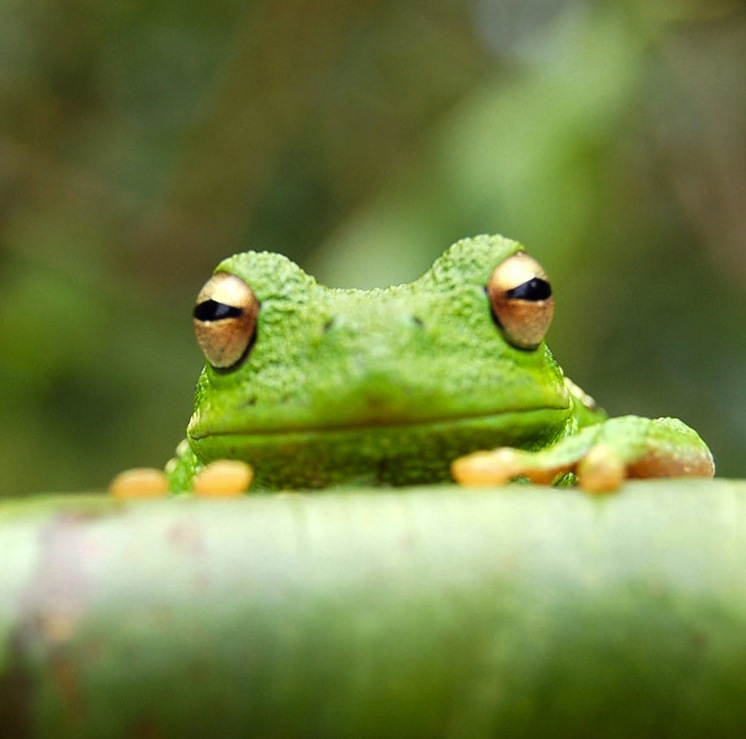
\includegraphics[width=0.3\textwidth]{Images/frog.jpg}
\caption{\label{fig:frog}This frog was uploaded via the file-tree menu.}
\end{figure}

\subsection{How to add Tables}

Use the table and tabular environments for basic tables --- see Table~\ref{tab:widgets}, for example. For more information, please see this help article on \href{https://www.overleaf.com/learn/latex/tables}{tables}. 

\begin{table}
\centering
\begin{tabular}{l|r}
Item & Quantity \\\hline
Widgets & 42 \\
Gadgets & 13
\end{tabular}
\caption{\label{tab:widgets}An example table.}
\end{table}

\subsection{How to add Comments and Track Changes}

Comments can be added to your project by highlighting some text and clicking ``Add comment'' in the top right of the editor pane. To view existing comments, click on the Review menu in the toolbar above. To reply to a comment, click on the Reply button in the lower right corner of the comment. You can close the Review pane by clicking its name on the toolbar when you're done reviewing for the time being.

Track changes are available on all our \href{https://www.overleaf.com/user/subscription/plans}{premium plans}, and can be toggled on or off using the option at the top of the Review pane. Track changes allow you to keep track of every change made to the document, along with the person making the change. 

\subsection{How to add Lists}

You can make lists with automatic numbering \dots

\begin{enumerate}
\item Like this,
\item and like this.
\end{enumerate}
\dots or bullet points \dots
\begin{itemize}
\item Like this,
\item and like this.
\end{itemize}

\subsection{How to write Mathematics}

\LaTeX{} is great at typesetting mathematics. Let $X_1, X_2, \ldots, X_n$ be a sequence of independent and identically distributed random variables with $\text{E}[X_i] = \mu$ and $\text{Var}[X_i] = \sigma^2 < \infty$, and let
\[S_n = \frac{X_1 + X_2 + \cdots + X_n}{n}
      = \frac{1}{n}\sum_{i}^{n} X_i\]
denote their mean. Then as $n$ approaches infinity, the random variables $\sqrt{n}(S_n - \mu)$ converge in distribution to a normal $\mathcal{N}(0, \sigma^2)$.


\subsection{How to change the margins and paper size}

Usually the template you're using will have the page margins and paper size set correctly for that use-case. For example, if you're using a journal article template provided by the journal publisher, that template will be formatted according to their requirements. In these cases, it's best not to alter the margins directly.

If however you're using a more general template, such as this one, and would like to alter the margins, a common way to do so is via the geometry package. You can find the geometry package loaded in the preamble at the top of this example file, and if you'd like to learn more about how to adjust the settings, please visit this help article on \href{https://www.overleaf.com/learn/latex/page_size_and_margins}{page size and margins}.

\subsection{How to change the document language and spell check settings}

Overleaf supports many different languages, including multiple different languages within one document. 

To configure the document language, simply edit the option provided to the babel package in the preamble at the top of this example project. To learn more about the different options, please visit this help article on \href{https://www.overleaf.com/learn/latex/International_language_support}{international language support}.

To change the spell check language, simply open the Overleaf menu at the top left of the editor window, scroll down to the spell check setting, and adjust accordingly.

\subsection{How to add Citations and a References List}

You can simply upload a \verb|.bib| file containing your BibTeX entries, created with a tool such as JabRef. You can then cite entries from it, like this: \cite{greenwade93}. Just remember to specify a bibliography style, as well as the filename of the \verb|.bib|. You can find a \href{https://www.overleaf.com/help/97-how-to-include-a-bibliography-using-bibtex}{video tutorial here} to learn more about BibTeX.

If you have an \href{https://www.overleaf.com/user/subscription/plans}{upgraded account}, you can also import your Mendeley or Zotero library directly as a \verb|.bib| file, via the upload menu in the file-tree.

\subsection{Good luck!}

We hope you find Overleaf useful, and do take a look at our \href{https://www.overleaf.com/learn}{help library} for more tutorials and user guides! Please also let us know if you have any feedback using the Contact Us link at the bottom of the Overleaf menu --- or use the contact form at \url{https://www.overleaf.com/contact}.

\bibliographystyle{alpha}
\bibliography{sample}

\end{document}